\chapter{TỔNG QUAN}
\label{s:tong_quan}
Nội dung chương đặt vấn đề tổng quan bài toán nhận dạng ngôn ngữ ký hiệu hiện nay và một số các công trình nghiên cứu về nhận dạng ngôn ngữ ký hiệu đã công bố trong nước và quốc tế. Từ đó đưa ra lý do chọn đề tài nhận dạng ngôn ngữ ký hiệu, giới thiệu về công cụ hỗ trợ cũng như mục tiêu, nhiệm vụ của đề tài cần tập trung giải quyết. Ngoài ra, chương mở đầu cũng giới thiệu phương pháp xử lý đề tài luận văn và trình bày bố cục nội dung trình bày xuyên suốt bài báo cáo.

\section{Đặt vấn đề}
Khiếm thính là trình trạng một người có thính giác kém, không nghe được những âm thanh, tiếng nói mà một người bình thường có thể nghe được. Theo số liệu thống kê năm 2014 của Trung tâm nghiên cứu Giáo dục đặc biệt (Viện Khoa học GD Việt Nam), Việt Nam có khoảng 7 triệu người khuyết tật, trong đó có hơn 1 triệu người khiếm thính. Do khả năng nghe bị suy giảm nên việc giao tiếp bằng lời nói ở cộng đồng người khiếm thính  và với người bình thường dường như là không thể. Để thay thế cho việc giao tiếp bằng tiếng nói, “ngôn ngữ ký hiệu” được ra đời nhằm phục vụ việc giao tiếp trực tiếp mà không cần thông qua lời nói.
Ngôn ngữ ký hiệu hay ngôn ngữ dấu hiệu, thủ ngữ là ngôn ngữ dùng những biểu hiện của bàn tay thay cho âm thanh của tiếng nói. Ngôn ngữ ký hiệu do người khiếm thính tạo ra nhằm giúp họ có thể giao tiếp với nhau trong cộng đồng của mình và tiếp thu tri thức của xã hội. Ngôn ngữ ký hiệu không như chữ viết tay hay lời nói có một cách thức và ngữ pháp cụ thể, ký hiệu rõ ràng để có thể mô hình hóa được. Để sử dụng ngôn ngữ ký hiệu, người giao tiếp cần thể hiện cử chỉ bằng cả bàn tay và cánh tay, kết hợp với điệu bộ của cơ thể để có thể diễn tả ý nghĩa mong muốn. Tuy được cộng đồng người khiếm thính sử dụng phổ biến nhưng đối với người bình thường, hầu như đa số đều không hiểu ngôn ngữ ký hiệu. Ngoài ra, ngôn ngữ ký hiệu giữa các nước trên thế giới, thậm chí giữa các vùng miền trong một nước cũng có sự khác nhau. Việc này khiến cho việc giao tiếp của người khiếm thính gặp rất nhiều khó khăn. Vì vậy một hệ thống nhận dạng ngôn ngữ ký hiệu tự động phiên dịch sang tiếng nói giúp người khiếm thính hòa nhập cộng đồng là thật sự cần thiết.
Với những lý do đó, trong đề cương này em xin trình bày một mô hình nhận dạng ngôn ngữ ký hiệu qua phân tích hình ảnh từ camera. Hệ thống này có khả năng quan sát, phát hiện con người và nhận diện hành động mà người đứng trước camera muốn diễn đạt. 

\section{Những nghiên cứu liên quan}
\label{ss:nghien_cuu_lien_quan}
Lĩnh vực xử lý, phân loại, nhận diện ngôn ngữ ký hiệu rất rộng và phức tạp do tính phong phú của chữ cái, câu từ và đặc tính không cấu trúc của các hành động con người. Các hướng phát triển trong lĩnh vực này rất tiềm năng và bùng nổ trong những năm gần đây.

Trên thế giới, đã có nhiều nghiên cứu phát triển các dịch vụ thông dịch ngôn ngữ ký hiệu và các sản phẩm công nghệ nhằm hỗ trợ người khiếm thính trong giao tiếp xã hội. Một số sản phẩm nổi bật như găng tay chuyển đổi ngôn ngữ ký hiệu thành giọng nói \cite{tl1}, các phần mềm dịch từ văn bản/ giọng nói sang ngôn ngữ ký hiệu hay các từ điển tra cứu ngôn ngữ ký hiệu online \cite{tl2}. Một số tác giả cũng đã nghiên cứu sử dụng thiết bị Kinect trong việc nhận dạng các con số và các ký tự chữ cái theo ký hiệu ngôn ngữ người câm \cite{tl3}, tuy nhiên việc nhận dạng là dựa trên ảnh tĩnh chưa có những giải pháp nhận dạng ảnh động theo như các ký hiệu hiệu ngôn ngữ tiếng Việt.

Ở các nước, các nhà nghiên cứu đã tiếp cận bài toán nhận dạng cử chỉ bàn tay theo rất nhiều hướng khác nhau như dựa vào màu sắc bàn tay, hình dáng bàn tay hay công trình của Viola $\&$ Jones dùng các đặc trưng Haarlike.

Ngoài ra, lĩnh vực nhận diện cử chỉ của con người được quan tâm và nghiên cứu trong rất nhiều năm từ năm 1992 \cite{Yamato} với giải thuật HMM của Junji YAMATO cho đến những năm gần đây, sử dụng phương pháp SVM cục bộ của Christian Schudlt vào năm 2004 \cite{Schuldt:2004:RHA:1018429.1020906}, và các phương pháp khác như: giải thuật khung xương \cite{Chen:2006:HAR:1178782.1178808}, \cite{Forsyth}, \cite{With}. Các bài khảo sát chi tiết có thể được tìm thấy ở \cite{Cristani201386} khảo sát cách thức nhận diện hành động con người và đưa ra chi tiết nhiều bài báo có thể tham khảo.

Như đã đề cập ở các phần trên, phương pháp SVM chỉ hoạt động tốt với các ảnh tĩnh, nên các nhận diện chính xác của SVM phải nói chính xác là các cử chỉ của con người tại thời điểm tức thời đó đã được nhận diện chính xác, không phải là một hành động gồm nhiều cử chỉ. Luận văn này bên cạnh SVM thì cũng tập trung nhiều vào HMM nên các bài báo liên quan đến SVM và HMM đều được xem xét kỹ, trong đó có một số phương pháp rất hay và có thể được xem xét:

\begin{itemize}
\item Xây dựng mô hình 3D dựa vào nhiều camera ở các vị trí khác nhau \cite{HLUT1}
\item Nhận diện hành động con người dựa trên mô tả các đặc trưng góc 3D \cite{6693448}
\item Sử dụng nhiều thiết bị được gắn trên người \cite{4650859}
\end{itemize}

Mặc dù đã được nghiên cứu trong thời gian dài, tuy nhiên do đặc điểm của việc nhận dạng hành động con người rất phức tạp và không có một cấu trúc rõ ràng dẫn đến việc rất khó áp dụng cho thực tế hoặc một lĩnh vực rộng rãi.

\section{Mục tiêu của luận văn}

Để có thể thực hiện việc nhận dạng ngôn ngữ ký hiệu, cần xác định được phương pháp thực hiện, lựa chọn các giải thuật hợp lý phù hợp với điều kiện thực tế và khả năng có thể ứng dụng cao nhất.
Phương án thực hiện được lựa chọn ban đầu có 3 phương án: 

Phương án 1: sử dụng thiết bị kinect để trích xuất hình dáng khung xương sau đó nhận dạng ngôn ngữ ideoký hiệu bằng thuật toán Hidden Markov Model từ chuỗi ký tự khung xương được trích xuất ra.

Phương án 2: Thực hiện xây dựng mạng kết hợp Convoluntion Neural Network kết hợp với Long Short Term Memory để nhận dạng hành động từ video.

Phương án 3: Trích xuất hình dáng khung xương từ từng frame ảnh 2D bằng mạng CNN để xuất ra tọa độ khung xương trên hệ tọa độ 2D. Sử dụng một mạng Deep neural network để nhận dạng ngôn ngữ ký hiệu từ chuỗi khung xương đó.

Ở phương án 1 việc sử dụng thiết bị kinect sẽ là quá cồng kềnh để có thể mang theo, và sử dụng trong đời sống hàng ngày. Mô hình HMM có thể là một mô hình máy học cổ điển, còn nhiều nhược điểm hơn so với các mô hình mới hiện nay. Ở phương án 2, để phân loại hành động, cần có tập dữ liệu lớn vì với mỗi góc nhìn khác nhau sẽ cho ra một ảnh khác nhau và với cùng một hành động sẽ cho ra những đặc trưng khác nhau, như vậy sẽ khó để có thể xây dựng mô hình này. Phương án 3 được chọn vì có nhiều ưu điểm hơn phương án 1 và 2. Vì tính khả thi có thể ứng dụng được trên các thiết bị có camera mà người sử dụng có thể mang đi như điện thoại thông minh.

Ứng dụng hướng tới hỗ trợ cộng đồng người người khiếm thính trong giao tiếp thường ngày nên việc đầu tiên cần hướng đến là tính tiện lợi và dễ sử dụng. Vì vậy thiết bị giúp hỗ trợ người khiếm thính cần có thể dễ dàng mang đi gọn nhẹ. Do đó mục tiêu luận văn hướng đến là thực hiện phần mềm để có thể hoạt động trên điện thoại thông minh. 

\section{Nội dụng luận văn}
Nội dụng luận văn sẽ hướng đến xây dựng phần mềm nhận diện một số từ ngữ trong bộ ngôn ngữ ký hiệu của người khiếm thính ở TP.HCM. Các nội dụng này sẽ sắp xếp xoay quanh theo thứ tự hoạt động của mô hình nhận diện ngôn ngữ ký hiệu được xây dựng trong luận văn. Tổng quan, phần mềm nhận diện sẽ hoạt động theo các bước trong sơ đồ hình \ref{fig:diagram}.

\FloatBarrier
\begin{figure}[htp]
\begin{center}
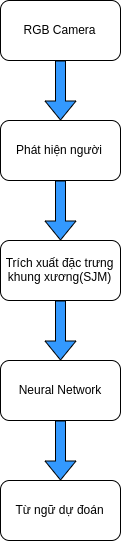
\includegraphics[scale=0.7]{chap1/c1_figs/diagram.png}
\end{center}
\caption{Thứ tự hoạt động mô hình nhận dạng}
\label{fig:diagram}
\end{figure}
\FloatBarrier


\section{Bố cục trình bày}
\label{ss:bo_cuc_trinh_bay}

Toàn bộ nội dung của luận văn sẽ đi theo bố cục chặt chẽ theo thứ tự các bước mà luận văn đã nghiên cứu và thực hiện. Các nội dung chính của luận văn sẽ được chia thành các chương cụ thể để có thể dễ dàng xem xét, và nắm bắt vấn đề. Tại mỗi chương sẽ trình bày cụ thể từ lý thuyết của chương đó cho đến cụ thể các bước thực hiện cũng như kết luận từng chương.

Bố cục của luận văn sẽ được trình bày theo trình tự và những nội dung được khái quát trong bảng \ref{table:bo_cuc_luan_van}.

\FloatBarrier
\begin{table}[h]
\caption{Tổng quan các chương của luận văn}
\label{table:bo_cuc_luan_van}
\centering
\begin{center}
\begin{tabular}{|c|p{13cm}|} 
 \hline
Chương  & Nội dung \\
 \hline
 Chương 1 & Giới thiệu chung về ngôn ngữ ký hiệu; Các nghiên cứu về nhận dạng ngôn ngữ ký hiệu; sơ lược mục tiêu, tổng quan và cấu trúc các phần của luận văn.\\
 \hline 
 Chương 2 & Trình bày lý thuyết về học sâu, các thuật toán huấn luyện mạng và mạng mobile net.\\
 \hline 
 Chương 3 & Giới thiệu các nghiên cứu về ước lượng đặc trưng khung xương; Cách thức hoạt động của mạng ước tính đặc trưng khung xương mà luận văn sử dụng .\\
 \hline
 Chương 4 & Trình bày về mạng neural network được luận văn xây dựng để phân loại các từ trong ngôn ngữ ký hiệu; Cách xử lý dữ liệu đầu vào của mạng và cách huấn luyện mạng. \\
 \hline 
 Chương 5 & Trình bày giải thuật Deep Sort dùng để theo dõi từng người trong khung hình.\\
 \hline
 Chương 6 & Xây dựng ứng dụng nhận diện dựa trên mô hình đã huấn luyện. Các thử nghiệm, kết quả và đánh giá mô hình. \\
 \hline
 Chương 7 & Trình bày kết luận và các hướng phát triển đề hoàn thiện đề tài.\\
 \hline
 
\end{tabular}
\end{center}
\end{table}
\FloatBarrier

